%**************** BASICS OF GEOMETRY ******************
\section{Basics of Differential Geometry}
In order to understand the Ricci Flow applications, it's necessary to study the properties of Riemannian Manifolds, in particular how to define a flow on a Manifold and how this is related to some differential equations. We'll see that the Ricci Flow is nothing but a differential equation for some class of different metrics on a Riemannian Manifold.


%***************** DIFFERENTIABLE MANIFOLDS ********************
\subsection{Differentiable Manfifolds}
Let's first refine the definition of a differentiable Manifold~\ref{def:manifold-prev}.

\begin{definition}[Differentiable manifold]
    $\M$ is an $n$-dimensional differentiable manifold if
    \begin{itemize}
        \item $\M$ is a topological space.
        \item $\M$ is provided with a family of pairs $\{ (U_i, \phi_i) \}$.
        \item $\{U_i\}$ is a family of open sets which covers $\M$, that is, $\cup_i U_i = \M$. $\phi_i$ is a homeomorphism from $U_i$ onto open subsets $U_i'$ of $\R^n$. See fig.~\ref{fig:homeomorphism}
        \item Given $U_i$ and $U_j$ such that $U_i \cap U_j \neq \emptyset$, the map $\psi_{ij} = \phi_i \circ \phi_j^{-1}$ from $\phi_j (U_i \cap U_j)$ to $\phi_i(U_i \cap U_j)$ is infinitely differentiable.
    \end{itemize}
\end{definition}

\begin{figure}
    \centering
    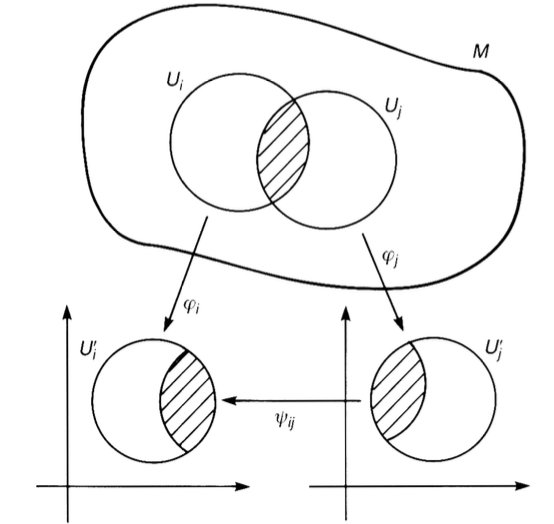
\includegraphics[width=0.5\textwidth]{Images/homeomorphism.png}
    \caption{$\phi_i$ is a homeomorphism from $U_i$ onto an open subset $U'_i$ of $\R^n$.}
    \label{fig:homeomorphism}
\end{figure}

The pair $(U_i, \phi_i)$ is called a \emph{chart}, while the whole family $\{(U_i, \phi_i)\}$ is an \emph{atlas}. The subset $U_i$ is called the \emph{coordinate neighbourhood}, while $\phi_i$ is the \emph{coordinate function}. This homeomorphism is represented by $n$ functions $\{x_1(p), \dots, x_n(p)\}$, which are called \emph{coordinates}. However, notice that a point $p\in\M$ is independent of its coordinates. In each coordinate neighbourhood $U_i$, $\M$ looks like an open subset of $\R_n$ whose element is $\{x^1, \dots x^n\}$, and this explains our previous definition~\ref{def:manifold-prev}.

Recall from the previous section that we're interested in Manifolds with boundaries. We're now able to define them.
\begin{definition}[Manifold with boundary]
    A \emph{Manifold with boundary} (see fig.~\ref{fig:boundary}) is a topological space $\M$ which is covered by a family of open sets $\{U_i\}$, each of which is homeomorphic to an open set of $H^n$, where
    \begin{equation}
        H^n \coloneq \{ (x^1, \dots, x^n) \in R^n | x^n \geq 0 \} .
    \end{equation} 
\end{definition}

\begin{figure}
    \centering
    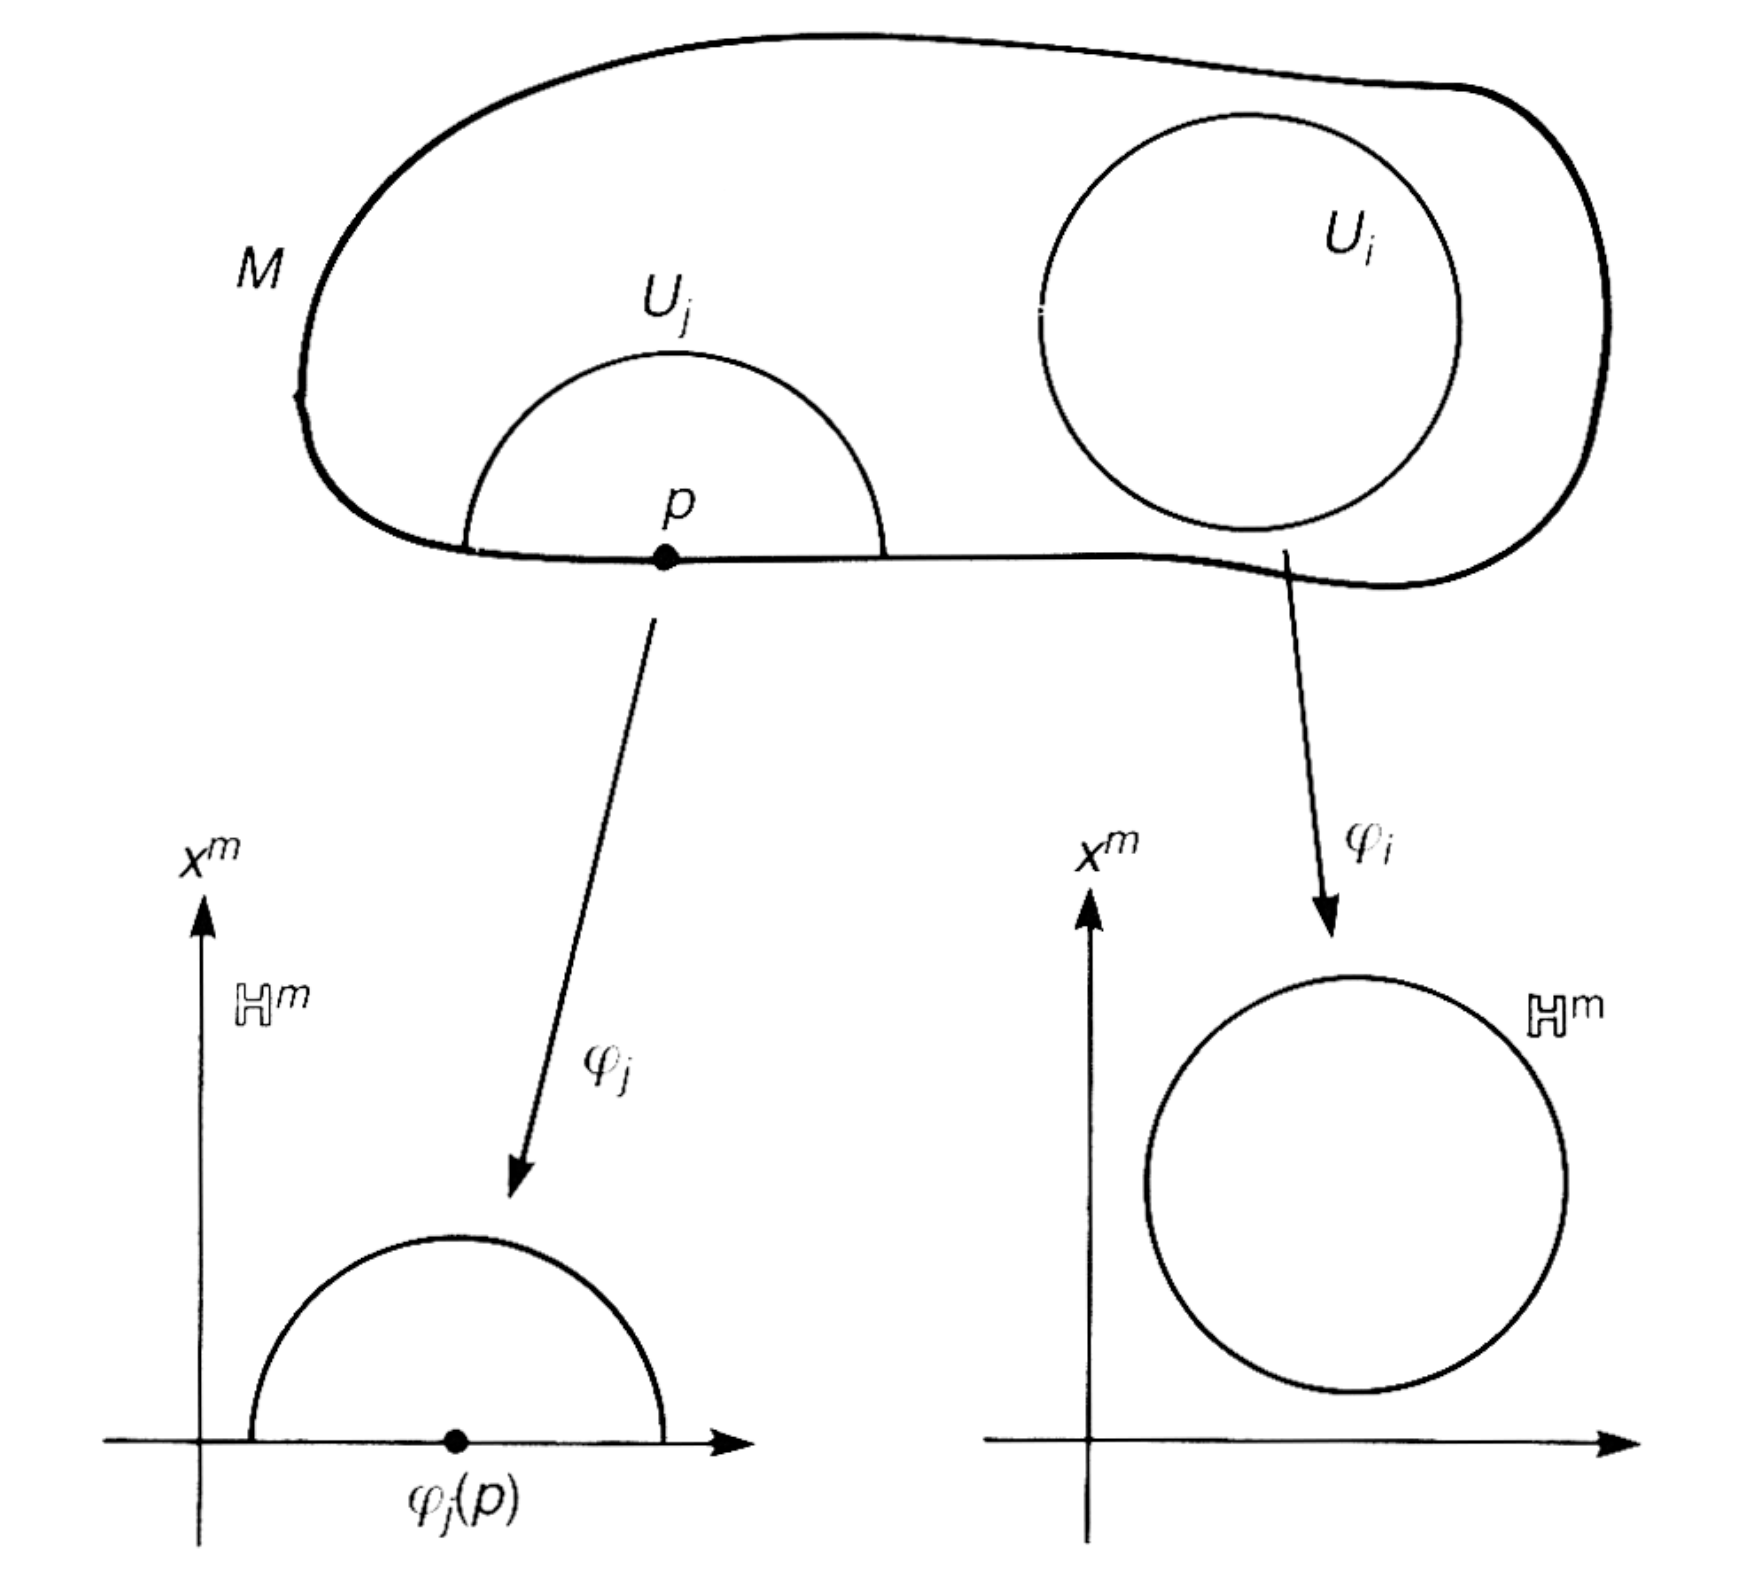
\includegraphics[width=0.5\textwidth]{Images/boundary.png}
    \caption{A Manifold $\M$ with boundary. Here, $p \in \de \M$.}
    \label{fig:boundary}
\end{figure}

The set of points which are mapped to points with $x_n = 0$ is called the \emph{boundary} of $\M$, denoted by $\partial \M$. The coordinates of $\partial \M$ may be given by $n-1$ numbers $(x^1, \dots, x^{n-1},0)$. One must then be careful to define smoothness. Indeed, the map $\psi_{ij} \colon \phi_j (U_i \cap U_j) \to \phi_i(U_i \cap U_j)$ is defined on an open set of $H^n$ in general, and $\phi_{ij}$ is said to be smooth if it's $C^\infty$ in an open set of $\R^n$ which contains $\phi_j(U_i \cap U_j)$.

%***************** DIFFERENTIABLE MAPS ********************
\subsection{Differentiable Maps}
Due to the presence of the differentiable structure on a Manifold, we're able to use the calculus techniques developed for $\R^n$. We can define a map between manifolds.

Let $\M$ and $\mathcal{N}$  be an $m$-dimensional and an $n$-dimensional Manifold, respectively. Let's then consider a map between them, i.e., $f: \M \to \mathcal{N}$, where $\M \ni p \mapsto f(p) \in \mathcal{N}$, see fig.~\ref{fig:map} Taking the charts $(U, \phi)$ on $\M$ and $(V,\psi)$ on $\mathcal{N}$,the coordinate representation of $f$ will be
\begin{equation}
    \phi \circ f \circ \phi^{-1}: \R^m \to \R^n .
\end{equation}
We can write $\phi(p) = \{x^\mu\}$ and $\psi(f(p)) = \{y^\alpha\}$, which makes explicit that $y \equiv \psi \circ f \circ \phi^{-1}(x)$ is an $m$-variables, vector-valued, usual function. Rendering the coordinate charts implicit, we may write $y^\alpha = f^\alpha(x^\mu)$, which makes clear why $f$ is said to be \emph{differentiable} at $p$ if $y$ is $C^\infty$. Notice, however, that the differentiability of $f$ is independent of the chosen coordinates.

\begin{figure}
    \centering
    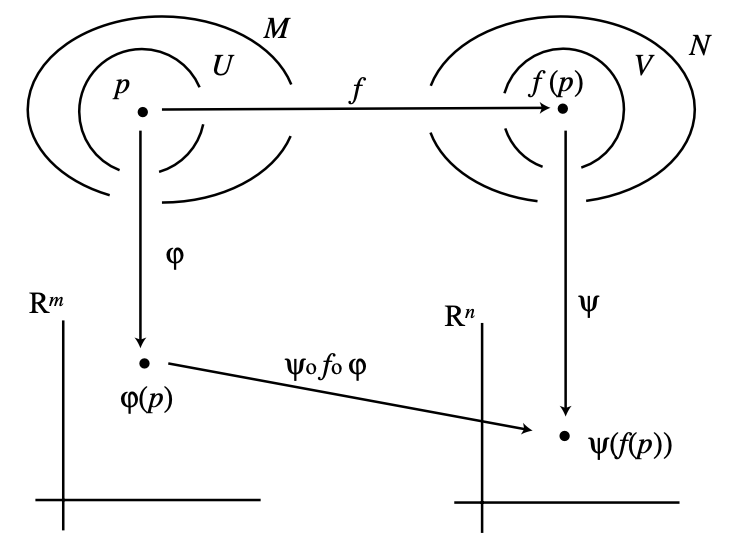
\includegraphics[width=0.5\textwidth]{Images/map.png}
    \caption{A map $f \colon \M \to \mathcal{N}$ has coordinates representation $\psi \circ f \circ \phi^{-1} \colon \R^m \to \R^n$.}
    \label{fig:map}
\end{figure}

A very important type of maps between manifold is given by diffeomorphisms.
\begin{definition}[Diffeomorphism]
    Let $f \colon \M \to \mathcal{N}$ be a homeomorphism and $\psi$ and $\phi$ the same coordinate functions as before. Then, if $\psi \circ f \circ \phi^{-1}$ is invertible and both $y \equiv \psi \circ f \circ \phi^{-1}(x)$ and $x \equiv \phi \circ f^{-1} \circ \psi^{-1}(y)$ are $C^\infty$, $f$ is called a \emph{diffeomorphism} and $\M$ is said to be \emph{diffeomorphic} to $\mathcal{N}$, $\M \equiv \mathcal{N}$.
\end{definition}

Taking a diffeomorphism from a Manifold into itself, we can implement the concept of change of coordinates, in two different interpretation. First, the set of diffeomorphisms $f\colon \M \to \M$ form a group denoted by $\diff(\M)$. Considering a particular $f \in \diff(\M)$, and a chart $(U, \phi)$, such that, for $p \in U$ and $f(p) \in U$, we get $\phi(p) = x^\mu(p)$ and $\phi(f(p))=y^\mu(f(p))$, then $y$ is a differentiable function of $x$ and the above diffeomorphism can be thought as an \emph{active transformation} for a change of coordinates.

However, if $(U,\phi)$ and $(V,\psi)$ are overlapping charts, for a point $p \in U \cap V$, there are two coordinates values, i.e., $x^\mu = \phi(p)$ and $y^\mu = \psi(p)$. Then, the map $x \mapsto y$ is differentiable, and it represents a \emph{passive transformation} for a change of coordinates.

Two important kinds of maps are curves and functions.

\begin{definition}[Curve]
    An \emph{open curve} in an $n$-dimensional Manifold $\M$ is a map $c \colon (a,b) \to \M$, where $(a,b)$ is an open interval such that $a<0<b$. A \emph{closed curve} is a map $c \colon S^1 \to \M$. On a chart $(U,\phi)$, a curve $c(t)$ ha the coordinate representation $x=\phi \circ c \colon \R \to \R^n$. See fig.~\ref{fig:curve}
\end{definition}

\begin{figure}
    \centering
    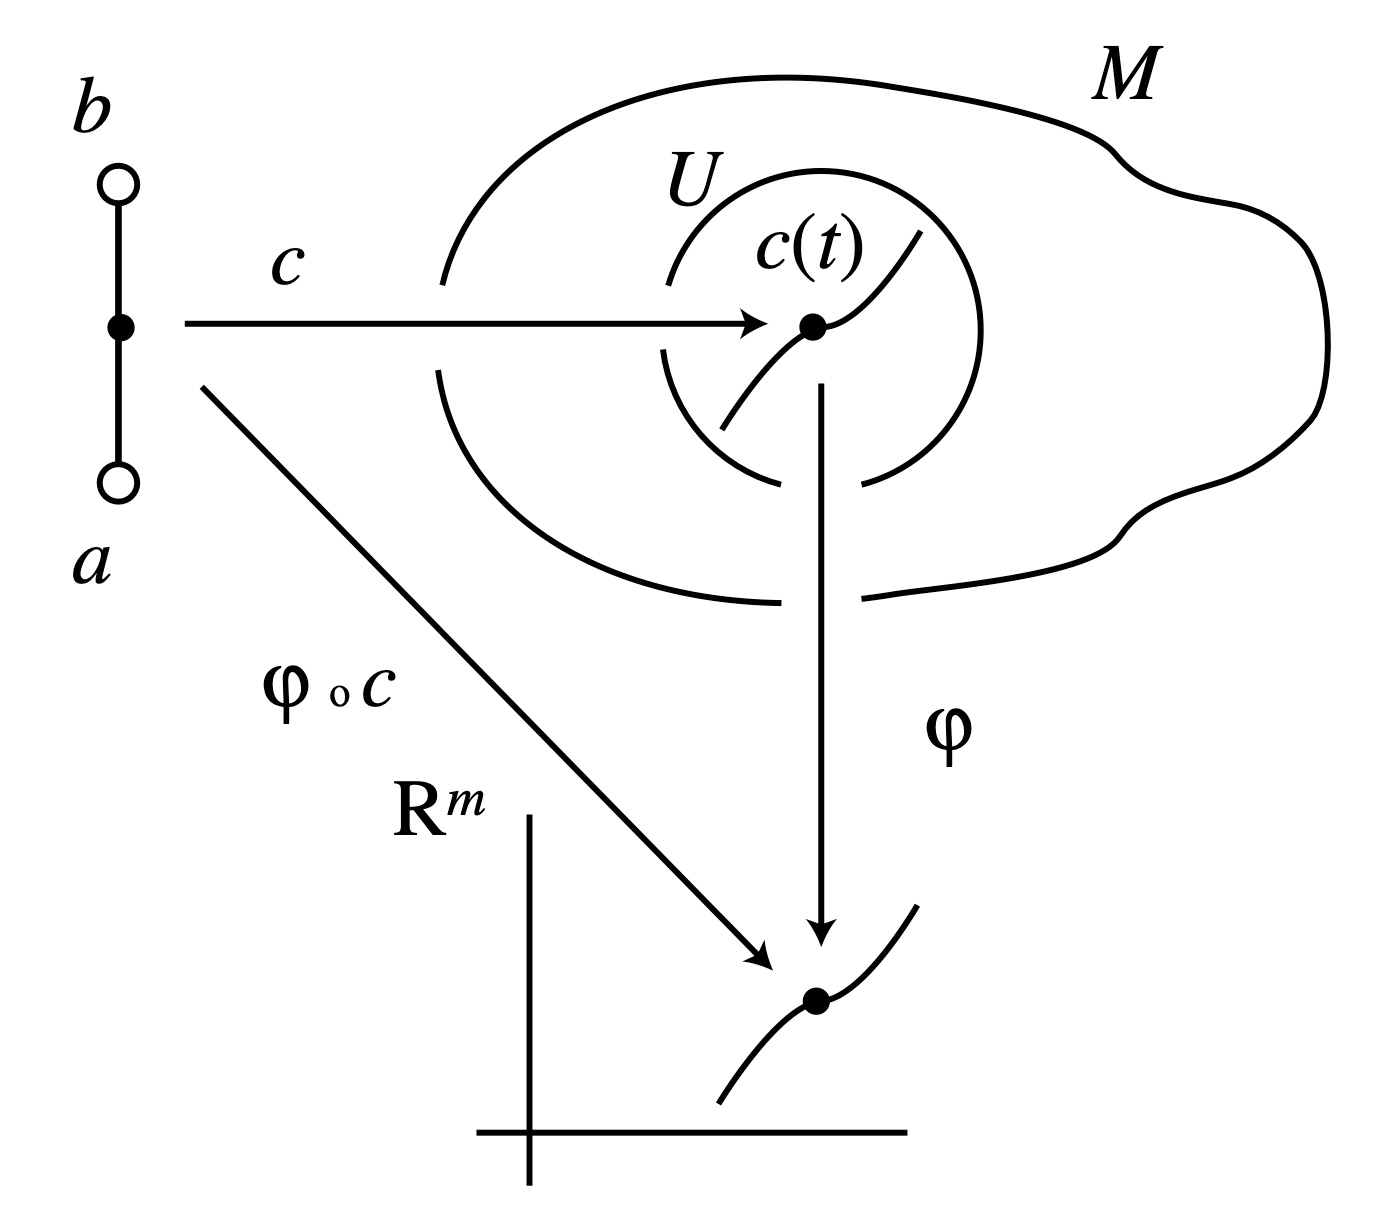
\includegraphics[width=0.5\textwidth]{Images/curve}
    \caption{A curve $c$ in $\M$ and its coordinate representation $\psi \circ c$.}
    \label{fig:curve}
\end{figure}

\begin{definition}[Function]
    A \emph{function} $f$ on $\M$ is a smooth map from $\M$ to $\R$. On a chart $(U,\phi)$, the coordinate representation of $f$ is given by $f \circ \phi^{-1} \colon \R^n \to \R$, which is a real-valued function of $n$ variables. The set of functions is denoted by $\mathfrak{F}(\M)$. See fig.~\ref{fig:function}
\end{definition}

\begin{figure}
    \centering
    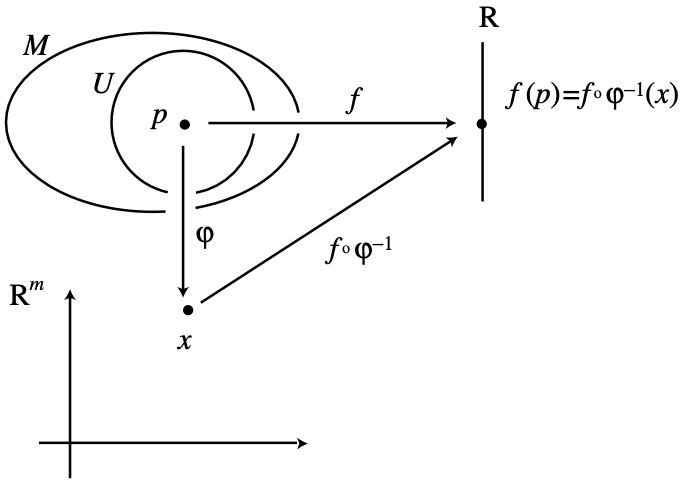
\includegraphics[width=0.5\textwidth]{Images/function.png}
    \caption{A function $f\colon \M \to \R$ and its coordinate representation $f \circ \phi^{-1}$.}
    \label{fig:function}
\end{figure}

%***************** VECTORS ********************
\subsection{Vectors}
The curves allow us to define a vector as a differential operator. So understand this more deeply, let's take a Manifold $\M$, a curve $c\colon (a,b) \to \M$ and a function $f \colon \M \to \R$, where $(a,b)$ is an open interval containing $t=0$, as showed in fig.~\ref{fig:vector}. The tangent vector at $c(0)$ is defined to be the directional derivative of a function $f(c(t))$ along the curve $c(t)$ at $t=0$. In particular,
\begin{equation}
    X[f] \coloneq \left. \frac{\ud f (c(t))}{\ud t}\right|_{t=0} = \left. \frac{\partial f}{\partial x^\mu} \frac{\ud x^\mu(c(t))}{\ud t} \right|_{t=0} = X^\mu \left(\frac{\de f}{\de x^\mu}\right),
\end{equation}
where we defined
\begin{equation}\label{eq:def-vectors}
    X = X^\mu \left(\frac{\de}{\de x^\mu}\right), \quad X^\mu = \left. \frac{\ud x^\mu(c(t))}{\ud t} \right|_{t=0}
\end{equation}
Notice that we used abuse of notation, that is $\de f / \de x^\mu$ really means $\de (f \circ \phi^{-1}(x))/\de x^\mu$.

\begin{figure}
    \centering
    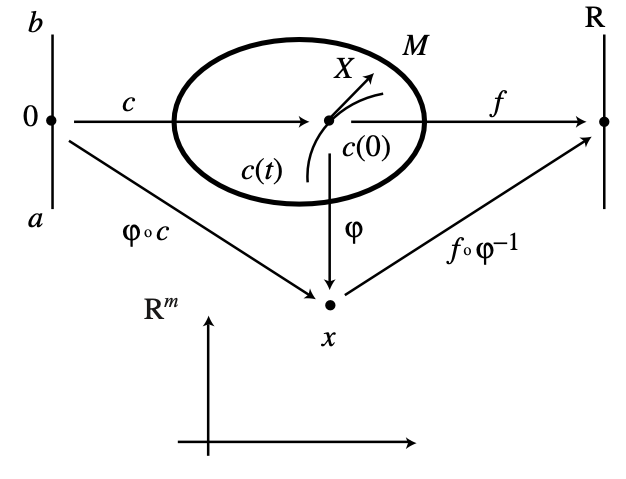
\includegraphics[width=0.5\textwidth]{Images/vector.png}
    \caption{A curve $c$ and a function $f$ define a tangent vector along the curve in terms of directional derivatives.}
    \label{fig:vector}
\end{figure}

Trying to be more precise, as known from multivariate analysis, whenever we have a curve, we can define an equivalence class. This case is no different. Indeed, given two curves $c_1(t)$ and $c_2(t)$ on $\M$, if they satisfy
\begin{subequations}
\begin{gather}
    c_1(0)= c_2(0)=p, \\
    \left. \frac{\ud x^\mu(c_1(t))}{\ud t} \right|_{t=0} = \left. \frac{\ud x^\mu(c_2(t))}{\ud t} \right|_{t=0} ,
\end{gather}
\end{subequations}
then they yield the same differential operator $X$ at $p$. Then, the above conditions define an equivalence relation $\sim$ such that $c_1(t) \sim c_2(t)$. This allows us to define
\begin{definition}[Vector]
    A \emph{tangent vector} $X$ is the \emph{equivalence class of curves}
    \begin{equation}
        [c(t)] = \left\{ \tilde{c}(t) \; \Big| \; \tilde{c}(0) = c(0) \; \land \; \left. \frac{\ud x^\mu (\tilde{c}(t))}{\ud t}\right|_{t=0} = \left. \frac{\ud x^\mu (c(t))}{\ud t}\right|_{t=0} \right\} .
    \end{equation}
\end{definition}
All the tangent vectors at a particular point $p \in \M$ form a vector space called \emph{tangent space} of $\M$ at $p$, denoted by $T_p \M$. By means of equation~\eqref{eq:def-vectors}, it's straightforward to see that the basis vectors of this vector space are
\begin{equation}
    \left\{ e_\mu = \frac{\de}{\de x^\mu} \right\}   , \quad \mu = 1, \dots, n.
\end{equation}
Clearly, $\dim T_p \M = \dim \M$. Further, for each $V \in T_p \M$, we can expand it as $V = V^\mu e_\mu = V^\mu \de_\mu$, and we call $V^\mu$ the components of $V$ with respect to the basis. 

Obviously, $\{e_\mu\}$ are not the only possible basis for the vector space $T_p \M$. Indeed, as known from linear algebra, an arbitrary linear combination $\hat{e}_i \coloneq A_i^\mu e_\mu$, with $A = (A_i^\mu) \in GL(n,\R)$, is a basis as well. In this case, $\{\hat{e}_i\}$ is called a \emph{non-coordinate basis}.

Further, given that a vector exists independently of its coordinates, we can take two coordinate charts, with a point in the intersection of their domains, i.e., $p \in U_i \cap U_j$, with $x = \phi_i(p)$ and $y = \phi_j (p)$. A generic vector $X \in T_p \M$ can be equivalently expanded as
\begin{equation}
    X = X^\mu \frac{\de}{\de x^\mu} = \tilde{X}^\mu \frac{\de}{\de y^\mu},
\end{equation}
which shows the relation of the components of a vector in two different charts, i.e,
\begin{equation}
    \tilde{X}^\mu = X^\nu \frac{\de y^\mu}{\de x^\nu}.
\end{equation}

%***************** ONE-FORMS ********************
\subsection{One-Forms}
Given that $T_p \M$ is a vector space, we can define its dual vector space, whose elements are linear functional from $T_p \M$ to $\R$. This space is called \emph{cotangent space}, is denoted by $T^*_p \M$, and their elements $\omega \colon T_p \M \to \R \in T^*_p \M$ are called \emph{one-forms}.

The simplest one-form is the \emph{differential} of a function $f \in \F(\M)$. Indeed, for a vector $V \in T_p \M$, its action on $f$ is
\begin{equation}
    V[f] = V^\mu \frac{\de f}{\de x^\mu} \in \R.
\end{equation}
So, we define the action of $\ud f \in T^*_p \M$ on a vector $V \in T_p \M$ by
\begin{equation}
    \scalar{\ud f}{V} \equiv V[f] = V^\mu \frac{\de f}{\de x^\mu} \in \R.
\end{equation}
In coordinates $x = \phi(p)$, the differential can be expanded as
\begin{equation}
    \ud f = \frac{\de f}{\de x^\mu} \ud x^\mu,
\end{equation}
which clearly shows that $\{ \ud x^\mu \}$ is a basis of $T^*_p \M$. In particular, it's the dual basis of $\{ \de_\mu \}$, since
\begin{equation}
    \scalar{\ud x^\mu}{\de_\mu} = \frac{\de x^\nu}{\de x^\mu} = \delta^\nu_\mu .
\end{equation}

It's now easy to consider generic one-forms $\omega \in T^*_p \M$ and generic vectors $V \in T_p \M$. Picking a coordinate basis for the tangent space and its dual basis for the cotangent one, we can expand $\omega = \omega_\mu \ud x^\mu$ and $V = V^\mu \de_\mu$. Then, as usual, we can define an \emph{inner product} $\scalar{.}{.}\colon T^*_p \M \times T_p \M \to \R$ by
\begin{equation}\label{eq:def-inner-product-vector-one-form}
    \scalar{\omega}{V} = \omega_\mu V^\mu \scalar{\ud x^\mu}{\de_\nu} = \omega_\mu V^\nu \delta^\mu_\nu = \omega_\mu V^\mu.
\end{equation}

Finally, analogously than before, we can pick two charts and a point in their domain's intersection, $p \in U_i \cap U_j$, so that
\begin{equation}
    \omega = \omega_\mu \ud x^\mu = \tilde{\omega}_\nu \ud y^\nu,
\end{equation}
with $x = \phi_i(p)$ and $y=\phi_j(p)$. Then, we can easily infer the transformation rule of a one-form under a change of coordinates, indeed,
\begin{equation}
    \ud y^\nu = \frac{\de y^\nu}{\de x^\mu} \ud x^\mu \implies \tilde{\omega}_\nu = \omega_\mu \frac{\de x^\mu}{\de y^\nu} .
\end{equation}

%***************** TENSORS AND TENSOR FIELDS ********************
\subsection{Tensors and Tensor Fields}
From multilinear algebra, it should be familiar that a \emph{tensor} of type $(p,q)$ is a multilinear map which maps $q$ elements of $T^*_p \M$ and $r$ elements of $T_p \M$ to a real number:
\begin{equation}
    T^{(q,r)} \colon 
    \underbrace{T^*_p \M \otimes \dots \otimes T^*_p \M}_\text{$q$ times}
    \otimes
    \underbrace{T_p \M \otimes \dots \otimes T_p \M}_\text{$r$ times} \longrightarrow \R.
\end{equation}

Picking a coordinate basis and its dual basis,
\begin{equation}
    T^{(q,r)} = \tensor{T}{^{\mu_1}^\dots^{\mu_q}_{\nu_1}_\dots_{\nu_r}} \frac{\de}{\de x^{\mu_1}} \dots \frac{\de}{\de x^{\mu_q}} \ud x^{\nu_1} \dots \ud x^{\nu_r}.
\end{equation}

The set of type $(q,r)$ tensors at $p \in \M$ is denoted by $\Tau^q_{r;p}(\M)$. Further, taking $r$-vectors $V_a = V_a^\mu \de_\mu$ and $q$ one-forms $\omega_a = \omega_{a\mu} \ud x^\mu$,the action of $T^{(q,r)}$ on them is given by
\begin{equation}
    T(\omega_1, \dots, \omega_q; V_1, \dots, V_r) = \tensor{T}{^{\mu_1}^\dots^{\mu_q}_{\nu_1}_\dots_{\nu_r}} \omega_{1\mu_1} \dots \omega_{q\mu_q} V_1^{\nu_1} \dots V_r^{\nu_r}.
\end{equation}

In order to probe a Manifold structure, it's necessary to have fields defined in it, i.e., structures which are smoothly defined for each point of $\M$. Knowing the tensor structure at a point, it's easy to generalize it to the entire Manifold. To begin with, let's consider the simplest tensor, i.e., a vector, which is a $(1,0)$ tensor.

A \emph{vector field} is a vector assigned smoothly to each point of $\M$. In other words, $V$ is a vector field if $V[f] \in \F(\M)$, for any $f \in \F(\M)$. Then, each component of a vector field is itself a smooth function from $\M$ to $\R$. We denote the set of vector fields with $\X(\M)$. Then, a vector $X \in \X(\M)$ computed at a point $p \in \M$ is a vector at $T_p \M$, i.e., $X|_p \in T_p \M$.

Similarly, a \emph{tensor field} of type $(q,r)$ is a smooth assignment of an element of $\Tau^q_{r;p}(\M)$ at each point $p \in \M$. The set of tensor fields of type $(q,r)$ on $\M$ is denoted by $\Tau^q_r(\M)$.

An important tensor field we're interested in is the metric tensor, which is tightly related to the definition of a Ricci Flow, in the context of Riemannian Manifolds. However, let's first study an important property of vector fields: they can generate a flow on a Manifold. Studying further the relation among flows and differential equation, allows us to better grasp the definition of a Ricci Flow.

%***************** FLOW BY VECTOR FIELD ********************
\subsection{Flow generated by a vector field}
Let $X$ be a vector field in $\M$, $X \in \X(\M)$. An \emph{integral curve} $x(t)$ of $X$ is a curve in $\M$, whose tangent vector at $x(t)$ is $X|_x$. In a chart $(U,\phi)$, this is equivalent to
\begin{equation}\label{eq:ode-integral-curve}
    \frac{\ud x^\mu}{\ud t} = X^\mu(x(t)) ,
\end{equation}
where $x^\mu(t)$ is the $\mu$-th component of $\phi(x(t))$ and $X = X^\mu \de_\mu$. Pay attention to the abuse of notation. Indeed, we used $x$ to denote both a point on $\M$ and its coordinates.

Then, to finding the integral curve of a vector field $X$ is equivalent to solving the system of ODEs~\eqref{eq:ode-integral-curve}, with initial condition $x^\mu_0 = x^\mu (0)$, which are the coordinates of the integral curve at $t=0$.

The existence and uniqueness theorem of ODEs guarantees that there is a unique solution to~\eqref{eq:ode-integral-curve}, at least locally, with the initial condition $x^\mu_0$.

Let, then, $\sigma(t,x_0)$ be an integral curve of $X$ passing through a point $x_0$ at $t=0$ and let's denote its coordinates by $\sigma^\mu(t,x_0)$. Then, eq.~\eqref{eq:ode-integral-curve} becomes
\begin{equation}\label{eq:ode-flow-coordinates}
    \frac{\ud}{\ud t} \sigma^\mu (t,x_0) = X^\mu (\sigma(t,x_0)),
\end{equation}
with the initial condition
\begin{equation}\label{eq:ode-flow-initial-condition}
    \sigma^\mu(0,x_0) = x^\mu_0.
\end{equation}

The map $\sigma \colon \R \times \M \to \M$ si called \emph{flow} generated by $X \in \X(\M)$. We can prove it satisfies the condition
\begin{equation}\label{eq:property-flow}
    \sigma(t, \sigma^\mu(s,x_0)) = \sigma(t+s,x_0),
\end{equation}
for $s,t \in \R$.

\begin{proof}
    Since
    \begin{align*}
        \frac{\ud}{\ud t} \sigma^\mu (t, \sigma^\mu(s,x_0)) &= X^\mu (\sigma(t, \sigma^\mu(s,x_0))), \\
        \sigma(0,\sigma(s,x_0)) &= \sigma(s,x_0),
    \end{align*}
    and
    \begin{align*}
        \frac{\ud}{\ud t} \sigma^\mu (t+s,x_0) &= \frac{\ud}{\ud(t+s)} \sigma^\mu(t+s,x_0) = X^\mu(\sigma(t+s,x_0)), \\
        \sigma(0+s,x_0) &= \sigma(s,x_0),
    \end{align*}
    both sides of eq.~\eqref{eq:property-flow} satisfy the same ODE and the same initial condition. Then, from the uniqueness theorem for the solution of ODEs, they must be the same.
\end{proof}

This leads to the following theorem.
\begin{theorem}
    For any point $x \in \M$, there exists a differentiable map $\sigma \colon \R \times \M \to \M$ such that
    \begin{itemize}
        \item $\sigma(0,x) = x$;
        \item $t \mapsto \sigma(t,x)$ is a solution of~\eqref{eq:ode-flow-coordinates} and~\eqref{eq:ode-flow-initial-condition};
        \item $\sigma(t,\sigma^\mu(s,x)) = \sigma(t+s,x)$.
    \end{itemize}
\end{theorem}

We're now ready to introduce Riemannian Manifold and their most relevant properties.

%***************** METRIC TENSOR ********************
\subsection{Riemannian Manifolds}
A Riemannian Manifold is defined as a smooth Manifold which admits a Riemannian metric.

\begin{definition}
    Let $\M$ be a differentiable Manifold. A \emph{Riemannian metric} $g$ on $\M$ is a type $(0,2)$ tensor field on $\M$ such that, at each point $p \in \M$:
    \begin{itemize}
        \item $g_p (U,V) = g_p (V,U)$,
        \item $g_p(U,V) \geq 0$, where the equality holds only when $U=0$.
    \end{itemize}
    Here, $U,V \in T_p \M$ and $g_p = g|_p$. Basically, $g_p$ is a symmetric positive-definite bilinear form.
\end{definition}

Recall the previous definition of inner product~\eqref{eq:def-inner-product-vector-one-form} between vectors and dual forms. For $V \in T_p \M$ and $\omega \in T^*_p \M$, then $\scalar{.}{.} \colon T^*_p \M \times T_p \M \to \R$. If there exists a metric tensor $g$, then, we can use it to define the inner product between two vectors $U,V \in T_p \M$, specifically by $g_p(U,V)$. Since $g_p \colon T_p \M \otimes T_p \M \to \R$, we may define a linear map $g_p(U,.) \colon T_p \M \to \R$ by $V \mapsto g_p(U,V)$. Then, it's straightforward that $g_p(U,.) \in T^*_p \M$ is a one-form. Thus, the metric $g_p$ gives rise to an isomorphism between $T_p \M$ and $T^*_p \M$.

Picking a chart $(\phi,U)$, with coordinates $\{ x^\mu \}$, we can expand the metric tensor in coordinates as
\begin{equation}
    g_p = g_{\mu\nu}(p) \ud x^\mu \otimes \ud x^\nu, \quad g_{\mu\nu}(p) = g_p (\de_\mu, \de_\nu) = g_{\nu\mu}(p), \quad p \in \M.
\end{equation}

It's usual convention to forget about the point $p$, denote the inverse metric as $g^{\mu\nu}$, and the determinant as $\det(g_{\mu\nu}) \coloneq g$ and $\det(g^{\mu\nu}) \coloneq g^{-1}$. Then, the isomorphism between $T_p \M$ and $T^*_p \M$ can be expressed as
\begin{equation}
    \omega_\mu = g_{\mu\nu} U^\nu, \quad U^\mu = g^{\mu\nu} \omega_\nu .
\end{equation}

The purpose of the next chapter will be to rigorously define the Ricci Flow. However, to conclude this motivation part, let's take a brief detour onto string theory, in which, with a simple example in the context of non-linear sigma models, it's possible to grasp the meaning of the Ricci Flow application to understand topological properties of a Manifold through renormalization group flows in a Riemannian Manifold.